\chapter{State of the Art}
\label{chapter:State of the Art}

\begin{introduction}
This chapter will provide a comprehensive review of current \ac{5G} and Wi-Fi integration efforts, existing authentication mechanisms, and challenges in device identification, authentication and authorization. It will also explore recent developments and proposed solutions in the field, setting the context for our research.
\end{introduction}

\section{Why \acs{4G} needed improved security?}

From the point of view of authentication, a cellular network consists of three main components (see Figure \ref{fig:4G Cellular Network Architecture}): \ac{UE}, a \ac{SN}, and a \ac{HN}.

The \ac{UE} refers to devices like smartphones, tablets, or IoT devices equipped with a \ac{UICC}  hosting at least a \ac{USIM} storing security related artifacts, including a cryptographic key that is shared with the subscriber’s home network. These devices connect to the network over radio signals. In \acf{4G} \ac{LTE} networks, these signals utilize specific frequency bands allocated for \ac{4G} communication.

The \ac{SN} includes network components that establish communication and provide services to the \ac{UE} in a specific geographic area. Key elements of the \ac{SN} are the \ac{eNodeB} and the \ac{MME}.

\begin{itemize}
    \item{
        The \ac{eNodeB} is a base station that manages the radio connection between the \ac{UE} and the network. It handles tasks like scheduling radio resources, modulating and demodulating signals, and ensuring reliable data transmission over the air interface.
    }
    \item {
        The \ac{MME} is a core network element responsible for managing signaling between the \ac{UE} and the core network. It plays a key role in tasks such as authenticating the user, establishing bearers (data pathways), and ensuring mobility by managing handovers between \acp{eNodeB} as the \ac{UE} moves.
    }
\end{itemize}

The \ac{HN} refers to the network operated by the user's mobile service provider (e.g., MEO, Vodafone, or NOS). Among other functions, it stores subscriber information in a database called the \ac{HSS}.

\begin{itemize}
    \item {
        The \ac{HSS} is a critical component that contains subscription-specific data, such as subscription profiles, service entitlements, and cryptographic keys. These keys are used during the authentication process to verify and authorize, under specific conditions, access to that user in the network. The \ac{HSS} communicates with the \ac{SN} to authenticate the \ac{UE} using protocols like Diameter over an IP-based system. This ensures secure and efficient exchange of authentication and session-related information.
    }
\end{itemize}

Together, these core components form the \ac{EPS}~\cite{cbl-comp-p3}, the architecture underlying \ac{4G} \ac{LTE} networks. The \ac{EPS} enables seamless connectivity and service delivery by integrating the radio access network (\acp{eNodeB}) with the core network components (e.g., \ac{MME} and \ac{HSS}). This design ensures that authentication, data management, and mobility are handled efficiently while providing high-speed, low-latency connections for the \ac{UE}.

\begin{figure}
    \centering
    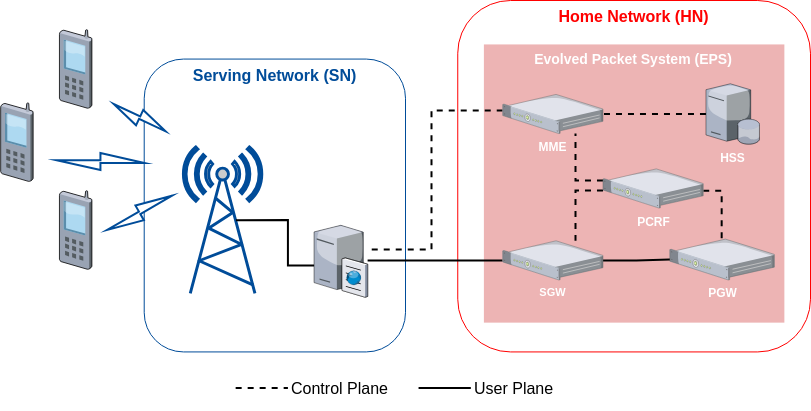
\includegraphics[width=0.75\linewidth]{figs/4G Cellular Network Architecture.png}
    \caption{\ac{4G} Cellular Network Architecture}
    \label{fig:4G Cellular Network Architecture}
\end{figure}

Communication between the \ac{SN} and \ac{HN} over the IP network is facilitated by core network protocols. The \ac{SN} sends a request to the \ac{HSS} containing the \ac{UE}’s credentials (e.g., \ac{IMSI}). The \ac{HSS} uses its stored keys to generate authentication vectors, which are then sent back to the \ac{SN}. The \ac{SN} uses these vectors to authenticate the \ac{UE} and establish a secure connection.

Prior generations to \ac{4G}, especially in \acp{RAN}, have faced significant security and privacy challenges. One major issue was the lack of network authentication in \ac{2G}~\cite{cbl-comp-p1}, which allowed attackers to perform network spoofing using fake base stations. For example, a fake base station could advertise a stronger signal and lure \ac{UE} away from its legitimate network, enabling the attacker to send fraudulent text messages to the user.

Another issue was the lack of integrity protection for signaling messages~\cite{cbl-comp-p1}, which left them vulnerable to spoofing and tampering. For instance, fake base stations could send unprotected Identity Request messages (a \ac{NAS} signaling message in \ac{LTE}) to steal permanent \ac{UE} identifiers, such as the \ac{IMSI}.

Additionally, certain messages lacked confidentiality~\cite{cbl-comp-p1}, resulting in privacy violations. For example, unencrypted paging messages could be intercepted to detect a user’s presence and track their precise location. 

To mitigate these vulnerabilities, the \ac{3GPP} introduced the \ac{AKA} protocol, which ensures entity authentication, message integrity, and message confidentiality. \ac{AKA} employs a challenge-response mechanism based on a symmetric key shared between the subscriber and their home network which is pre stored at the \ac{UE} in the \ac{UICC}/\ac{USIM} and in the network at the \ac{HSS}. It also derives cryptographic keying materials to protect both signaling messages and user plane data, including communications over radio channels. This protocol significantly enhances security and privacy in mobile networks.

In \ac{4G} \ac{EPS-AKA}, despite the enhancements brought by the \ac{3GPP} \ac{AKA} protocol, two significant flaws remain. First, during the initial stage of the authentication process (the flow is shown in Figure \ref{fig:4G-authentication-procedure}), the \ac{UE} must transmit its identity, specifically its \ac{IMSI}, to the serving network. This identity is sent over the radio network without encryption, leaving it vulnerable to interception~\cite{cbl-comp-p3}. Although the use of a temporary identifier, such as the \ac{GUTI}, is intended to mitigate this risk~\cite{eleftherakis-2024}, researchers have demonstrated that \ac{GUTI} allocation is flawed in that the identifiers either do not change frequently enough~\cite{gt-freq} or are assigned in predictable patterns~\cite{gt-pred}.

Second, during the authentication decision, the home network may provide an \ac{AV}, but this value is not directly included in the decision-making process, which is handled solely by the serving network~\cite{cbl-comp-p4}.

\begin{figure}[htbp]
    \centering
    \includegraphics[width=0.75\textwidth]{figs/4G-authentication-procedure.png}
    \caption{\ac{4G} Authentication Procedure}
    \label{fig:4G-authentication-procedure}
\end{figure}

\section{\acs{5G} Architecture and Security Framework}

The \ac{5G} System architecture, presented in Figure \ref{fig:5G-system-architecture}, is designed to exploit advanced techniques such as \ac{NFV} and \ac{SDN}. Besides, it separates \ac{CP} and \ac{UP} functions, enabling independent scalability, evolution, and flexible deployments in centralized or distributed locations. The architecture adopts a modular function design to support efficient network slicing and defines procedures as reusable services to enhance flexibility and can be easily extended. It minimizes dependencies between the \ac{AN} and the \ac{CN} by integrating different access types, including \ac{3GPP} and non-\ac{3GPP}, through a converged \ac{CN}.

\begin{figure}
    \centering
    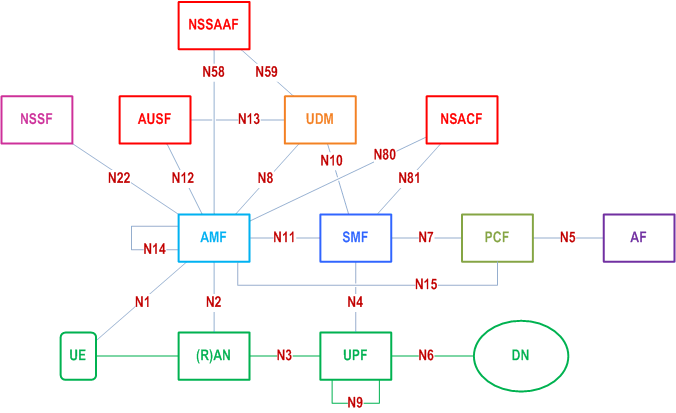
\includegraphics[width=0.75\linewidth]{figs/5g-system-architecture.png}
    \caption{Non-Roaming \acs{5G} System Architecture}
    \label{fig:5G-system-architecture}
\end{figure}

The system includes a unified authentication framework, supports stateless \acp{NF} by decoupling compute and storage resources, and enables capability exposure for network features. It allows concurrent access to local and centralized services and deploys \ac{UP} functions near the \acl{AN} to support low latency services and local data network access. Additionally, it supports roaming with both home-routed and local breakout traffic in visited networks, ensuring efficient and flexible operation~\cite{23.501-p41}.

In \ac{5G}, the security framework is built around a new way of organizing the network, known as \ac{SBA}. This setup introduces new entities~\cite{33.501-p30} and processes that focus on keeping the network secure, especially when it comes to authentication, which is the process of verifying users and devices.

\begin{itemize}
    \item{
        One of the key entities is the \ac{SEAF}, which is part of the \ac{AMF}, located in the serving network, acting as an intermediary during the authentication process~\cite{23.501-p48}. The \ac{SEAF} receives authentication requests from a device (\ac{UE}), but it relies on the home network to decide whether the authentication is valid or not. It can reject the authentication, but the final decision rests with the home network.
    }
    \item{
        The \ac{AUSF}~\cite{23.501-p538} is the entity in the home network that actually decides whether the device should be allowed into the network. The \ac{AUSF} looks at the information provided by the device and checks it against the home network's security policies. It then works with other backend services to compute the necessary data and keys needed to authenticate the device, using secure methods like \acf{5G-AKA} or \acf{EAP-AKA'}.
    }
    \item{
        The \ac{UDM}~\cite{23.501-p538} is in charge of managing the data involved in authentication. One of its key roles is managing the \ac{ARPF}, which selects the right authentication method based on the device's identity and the network's policies. It also helps generate the keys and data that the \ac{AUSF} uses for authentication.
    }
    \item{
        Finally, the \ac{SIDF}, which is part of the \ac{UDM}, helps protect the \ac{SUPI}. In \ac{5G}, this permanent identity, which could be a user’s \ac{IMSI}, is always kept hidden and encrypted when sent over the air to prevent hackers from tracking it. The \ac{SIDF} is the only part of the network that can decrypt the encrypted identity~\cite{33.501-p37} (called the \ac{SUCI}) using a private key, ensuring that no one else can access the user’s personal details.
    }
\end{itemize}

At its core, this framework introduces a unified and flexible authentication system that seamlessly integrates both \ac{3GPP} (traditional cellular) and non-\ac{3GPP} (such as Wi-Fi or cable) networks. This cross-network compatibility is crucial for enabling a wide range of access methods and supporting the growing ecosystem of connected devices.

Central to this framework is the \ac{EAP}, which facilitates secure communication between the \ac{UE} and the \ac{AUSF}. The \ac{SEAF} acts as an intermediary, relaying authentication messages between the \ac{UE} and \ac{AUSF}~\cite{33.501-p46}. This setup supports various authentication methods, including \ac{5G-AKA}, \ac{EAP-AKA'}, and \ac{EAP-TLS}, providing robust security for data exchange.

\subsection{Comparing \acs{5G-AKA}, \acs{EAP-AKA'} and \acs{EAP-TLS}}

\begin{figure}
    \centering
    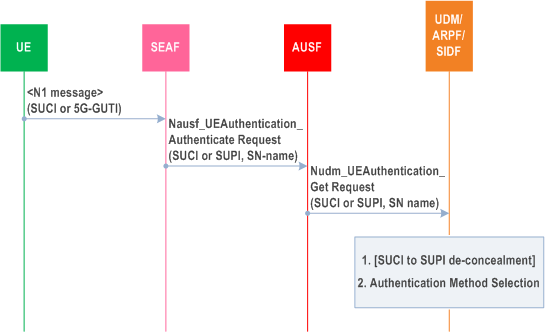
\includegraphics[width=0.75\linewidth]{figs/Initiation of authentication procedure and selection of authentication method.png}
    \caption{Initiation of authentication procedure and selection of authentication method}
    \label{fig:Initiation of authentication procedure and selection of authentication method}
\end{figure}

The \ac{5G-AKA} authentication process begins when the \ac{SEAF} receives a request from the \ac{UE} seeking network access (see Figure \ref{fig:Initiation of authentication procedure and selection of authentication method}). The \ac{UE} provides either a \acf{5G-GUTI} or a \ac{SUCI} to begin the authentication. The \ac{AUSF} first ensures that the requesting \ac{SN} is legitimate, then it sends an authentication request to the \ac{UDM}/\ac{ARPF}. If the \ac{SUCI} is provided, the \ac{SIDF} decrypts it to obtain the \ac{SUPI}, which is used to determine the authentication method~\cite{33.501-p48}.

\begin{figure}
    \centering
    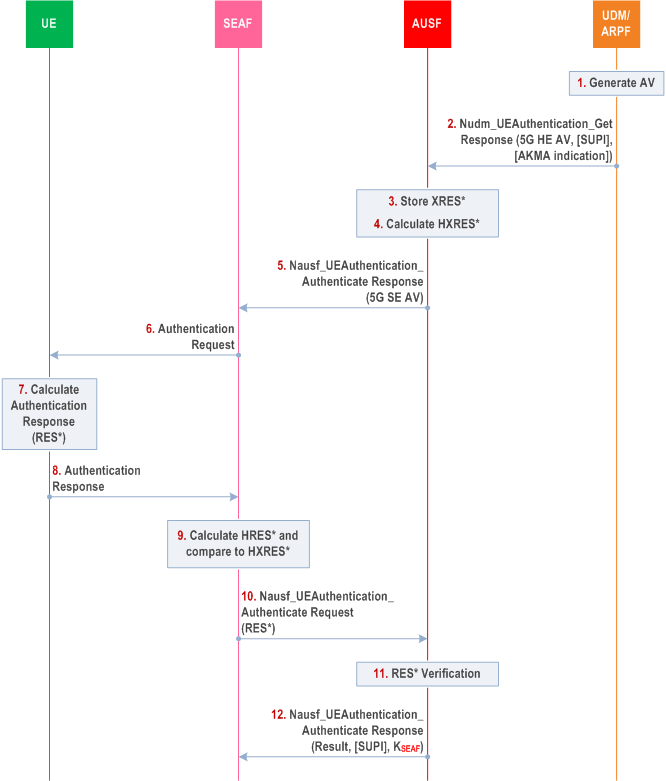
\includegraphics[width=0.75\linewidth]{figs/Authentication procedure for 5G AKA.png}
    \caption{Authentication procedure for \ac{5G-AKA}}
    \label{fig:Authentication procedure for 5G AKA}
\end{figure}

Next the \ac{UDM}/\ac{ARPF} generates an authentication response containing tokens and keys (see Figure \ref{fig:Authentication procedure for 5G AKA} message 1). These are sent to the \ac{AUSF}(message 2), which computes a hash ($HXRES$) and checks the expected response (message 3). The \ac{AUSF} sends the authentication result, including the $AUTH$ token and $HXRES$, to the \ac{SEAF} (message 5), ensuring that the \ac{SUPI} is not exposed to the \ac{SEAF}, preserving privacy. The \ac{SEAF} forwards the $AUTH$ token to the \ac{UE} (message 6), which then validates it using a secret key shared with the home network (message 7). If successful, the \ac{UE} computes a $RES$ token and sends it back to the \ac{SEAF} (message 8). The \ac{SEAF} calculates the $HRES$ and compares it (message 9), and then forwards this to the \ac{AUSF} (message 10), which validates the response (message 11).

Once the $RES$ token is verified, the \ac{AUSF} sends an anchor key to the \ac{SEAF} (message 12). The \ac{SEAF} derives an \acs{AMF} key, which the \acl{AMF} uses to generate further keys for securing signaling messages between the \ac{UE} and network elements. The \ac{UE}, using its root key, can derive all necessary keys for secure communication with the network, ensuring mutual trust and security~\cite{33.501-p52}.

\begin{figure}
    \centering
    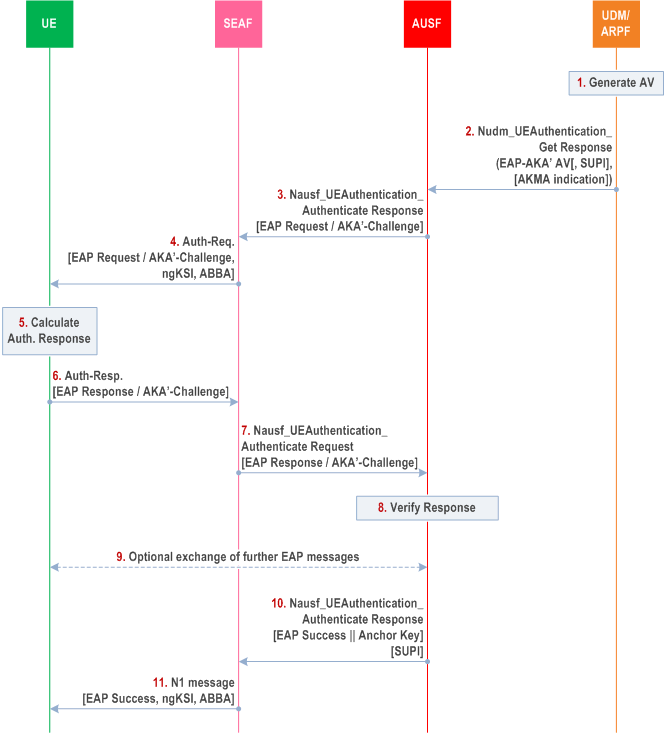
\includegraphics[width=0.75\linewidth]{figs/Authentication procedure for EAP-AKA'.png}
    \caption{Authentication procedure for \ac{EAP-AKA'}}
    \label{fig:Authentication procedure for EAP-AKA'}
\end{figure}

An alternative authentication method in \ac{5G} is \ac{EAP-AKA'}, which provides mutual authentication between the \ac{UE} and the network using a shared cryptographic key (see Figure \ref{fig:Authentication procedure for EAP-AKA'}). Unlike \ac{5G-AKA}, \ac{EAP-AKA'} uses \ac{EAP} messages within \ac{NAS} messages between the \ac{UE} and \ac{SEAF}, and between the \ac{SEAF} and \ac{AUSF}. In \ac{EAP-AKA'}, the \ac{SEAF} merely relays messages between the \ac{UE} and the \ac{AUSF} without making authentication decisions. In contrast, in \ac{5G-AKA}, the \ac{SEAF} verifies the \ac{UE}'s authentication response and can act on failures. The $K_{AUSF}$ key in \ac{5G-AKA} is generated by the \ac{UDM}/\ac{ARPF} and sent to the \ac{AUSF}, while in \ac{EAP-AKA'}, the \ac{AUSF} derives this key from the \ac{EMSK}, which is provided by \ac{UDM}/\ac{ARPF}~\cite{33.501-p49}.

\begin{figure}
    \centering
    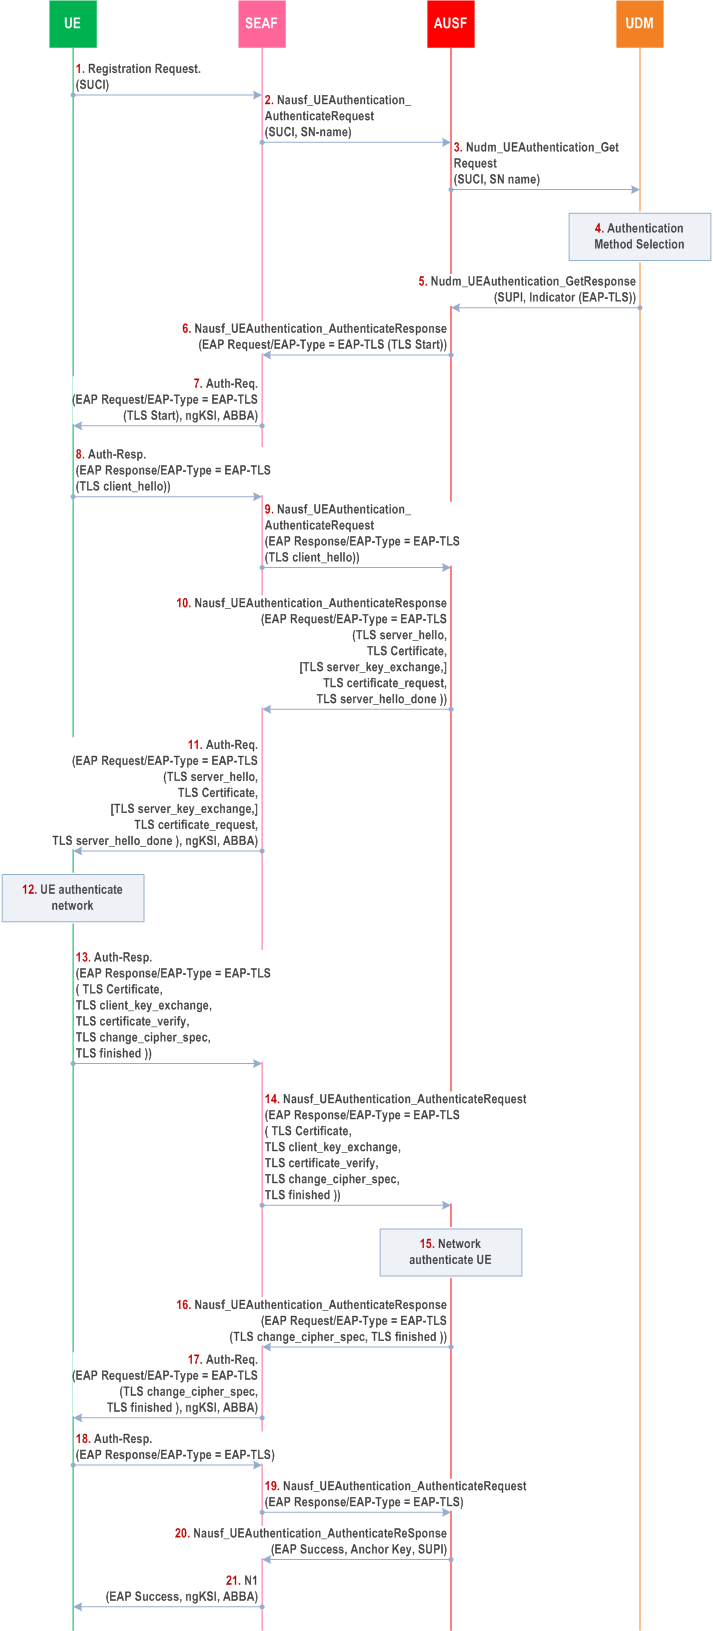
\includegraphics[width=0.5\linewidth]{figs/Using EAP-TLS Authentication Procedures over 5G Networks for initial authentication.png}
    \caption{Using \ac{EAP-TLS} Authentication Procedures over \ac{5G} Networks for initial authentication}
    \label{fig:Using EAP-TLS Authentication Procedures over 5G Networks for initial authentication}
\end{figure}

Additionally, \ac{EAP-TLS} (see Figure \ref{fig:Using EAP-TLS Authentication Procedures over 5G Networks for initial authentication}) is another optional authentication method suitable for specific scenarios such as private networks or \ac{IoT} devices. Like \ac{EAP-AKA'}, \ac{EAP-TLS} involves mutual authentication via public key certificates or a \ac{PSK}. The \ac{SEAF} acts as an \ac{EAP} authenticator, forwarding \ac{EAP-TLS} messages between the \ac{UE} and the \ac{AUSF}. This method differs from the \ac{AKA}-based approaches by relying on public key certificates for trust, eliminating the need for symmetric keys shared between the \ac{UE} and the network. This reduces key management risks and does not require a traditional \ac{USIM}, although secure elements are still needed for storing credentials~\cite{33.501-p232}.

\section{Identity Management in \acs{5G}}

In the transition to \ac{5G}, new mechanisms were introduced to address the vulnerabilities associated with exposed identifiers, such as the \ac{IMSI} (see Figure \ref{fig:International Mobile Subscriber Identity (IMSI)}), during \ac{RAN} communication. These enhancements ensure privacy, security, and compatibility with legacy systems.

\begin{figure}
    \centering
    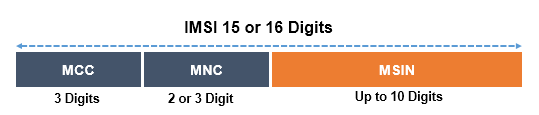
\includegraphics[width=0.75\linewidth]{figs/International Mobile Subscriber Identity (IMSI).png}
    \caption{\ac{IMSI}}
    \label{fig:International Mobile Subscriber Identity (IMSI)}
\end{figure}

One of those mechanisms is the \ac{SUPI}, which serves as the globally unique identifier for each subscriber within the \ac{5G} system. Designed for authentication and provisioning, the \ac{SUPI} maintains compatibility with legacy formats such as the \ac{IMSI} and \ac{NAI}~\cite{23.501-p243}. This flexibility ensures seamless interworking with older systems, including the \ac{EPC}.

The \ac{SUPI} is typically structured as follows:
\begin{itemize}
    \item {
        \ac{IMSI}-based \ac{SUPI}: Includes the \ac{MCC}, the \ac{MNC}, and the \ac{MSIN}~\cite{23.003-p20}.
    }
    \item {
        \ac{NAI}-based \ac{SUPI}: Uses an \ac{NAI} format (\texttt{username@realm}), offering support for scenarios requiring integration with external identity systems or non-\ac{3GPP} access.
    }
\end{itemize}

It is important to note that for interworking with \ac{EPC}, the \ac{SUPI} must be \ac{IMSI}-based, ensuring compatibility with existing \ac{LTE} systems and infrastructure.

Unlike its predecessor, the \ac{SUPI} is never transmitted in plaintext over the air. Instead, it is concealed as a \ac{SUCI} (see Figure \ref{fig:Subscription Concealed Identifier (SUCI)}) using an \ac{ECIES} and the home network’s public key. This encryption ensures the confidentiality of user identities during initial registration and subsequent communications.

\begin{figure}
    \centering
    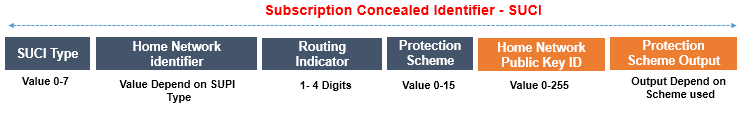
\includegraphics[width=0.75\linewidth]{figs/Subscription Concealed Identifier (SUCI).png}
    \caption{\ac{SUCI}}
    \label{fig:Subscription Concealed Identifier (SUCI)}
\end{figure}

The \ac{SUCI} construction includes:
\begin{itemize}
    \item{
        \textbf{\ac{SUPI} Type}: A value in the range 0 to 7. It identifies the type of the \ac{SUPI} concealed in the \ac{SUCI}. These could be an \ac{IMSI}, a \ac{NSI}, a \ac{GLI} or \ac{GCI}
    }
    \item{
        \textbf{Home Network Identifier}: Includes the \ac{MCC} and \ac{MNC} for routing purposes.
    }
    \item{
        \textbf{Routing Indicator}: 1 to 4 decimal digits, assigned by the home network operator and provisioned in the \ac{USIM}, that allow together with the Home Network Identifier to route network signalling with \ac{SUCI} to \ac{AUSF} and \ac{UDM} instances capable to serve the subscriber.
    }
    \item{
        \textbf{Protection Scheme ID}: Specifies the encryption method used.
    }
    \item{
        \textbf{Home Network Public Key ID}: Identifies the key applied for encryption.
    }
    \item{
        \textbf{Encrypted Scheme Output}: Represents the concealed \ac{SUPI}.
    }
\end{itemize}

The \ac{SUCI} computation is determined by the operator's policy stored in the \ac{USIM}. Depending on the configuration, the \ac{SUCI} may be calculated directly by the \ac{USIM} or delegated to the \ac{ME}~\cite{23.003-p21}.

An anonymous \ac{SUCI} is composed by setting the \ac{SUPI} Type field to 1 (Network-Specific Identifier), using the null protection scheme, and where the scheme output corresponds to a username set to either the "anonymous" string or to an empty string.

To further enhance privacy, \ac{5G} utilizes temporary identifiers during communication. The \acl{5G-GUTI}~\cite{23.501-p244}(see Figure \ref{fig:5G Global Unique Temporary Identifier (5G–GUTI)}) is dynamically assigned by the \ac{AMF} and replaces the \ac{SUPI} in subsequent signaling exchanges. This frequent reassignment minimizes the risk of user tracking.

\begin{figure}
    \centering
    \includegraphics[width=0.75\linewidth]{figs/5G Global Unique Temporary Identifier (5G–GUTI).png}
    \caption{\ac{5G-GUTI}}
    \label{fig:5G Global Unique Temporary Identifier (5G–GUTI)}
\end{figure}

The \ac{5G-GUTI} is typically in a format comprising:

\begin{enumerate}
    \item {
        \textbf{\ac{GUAMI}}: Identifies the \ac{AMF} managing the \ac{UE}'s session.
    }
    \item {
        \textbf{\ac{5G-TMSI}}: Uniquely identifies the \ac{UE} within the \ac{AMF} context.
    }
\end{enumerate}

For efficient radio signaling, a shortened version, the \ac{5G-S-TMSI}, is utilized. The \ac{5G-S-TMSI} is the shortened form of the \ac{GUTI} to enable more efficient radio signalling procedures (e.g. during Paging and Service Request)

Additionally, the \ac{5G-GUTI} can be represented in an \ac{NAI} format when required~\cite{23.003-p29}. This flexibility supports interworking and ensures compatibility across diverse network scenarios.

The \ac{AMF} retains the flexibility to assign new \ac{5G-GUTI} values at any time, though updates are generally synchronized with the next \ac{NAS} signaling exchange to avoid unnecessary interruptions. Despite these mechanisms, scenarios such as initial network access or failure to resolve a temporary identifier necessitate direct use of the \ac{SUPI}.

In addition to subscriber identifiers, the \ac{PEI} uniquely distinguishes user equipment capable of accessing the network. The \ac{PEI} is critical for device management but is safeguarded to prevent unauthorized tracking~\cite{23.501-p243}.

The \ac{PEI} adheres to specific formats based on device type and use case:
\begin{itemize}
    \item {
        For devices supporting \ac{3GPP} access, the \ac{IMEI} format is mandated, ensuring uniformity.
    }
    \item {
        The \ac{PEI} is presented with an indication of its format, enabling compatibility across diverse use cases.
    }
\end{itemize}

\section{Access Network Types in \acs{5G}}

\subsection{\acs{3GPP} vs non-\acs{3GPP}}
\ac{3GPP} encompasses standards for mobile networks like \ac{3G}, \ac{4G}, and \ac{5G}, which are cellular technologies enabling network services from mobile carriers. These networks operate on licensed spectrum, ensuring predictable performance, security, and quality of service.

In contrast, non-\ac{3GPP} access refers to technologies not standardized by \ac{3GPP}, such as Wi-Fi or satellite networks. These networks operate on unlicensed or partially licensed spectrum, are typically managed by different standards bodies (e.g., IEEE for Wi-Fi), and are widely used for cost-effective and ubiquitous connectivity~\cite{wba-04-2023-p3}. While non-\ac{3GPP} networks were previously considered external to mobile networks, \ac{5G} allows their tighter integration into the core network, enabling seamless user experiences across both network types.

\ac{5G} introduces the capability to support communication across both \ac{3GPP} and non-\ac{3GPP} access networks. This integration extends beyond traditional cellular devices, allowing a wide range of \acp{UE} and non-\acp{UE} devices—such as \ac{IoT} sensors, laptops, and legacy equipment—to connect securely and efficiently~\cite{23.501-p57}.

\ac{5G} supports communication across \ac{3GPP} and non-\ac{3GPP} access networks using distinct architectures for trusted and untrusted access. Trusted non-\ac{3GPP} networks rely on the \ac{TNGF} as seen in Figure \ref{fig:architecture-for-5g-core-network-with-trusted-non-3gpp-access}, while untrusted networks leverage the \ac{N3IWF} as seen in Figure \ref{fig:architecture-for-5g-core-network-with-untrusted-non-3gpp-access}. Both gateway functions connect to the \ac{5GC}’s control and user planes via the N2 and N3 reference points.

\begin{figure}
    \centering
    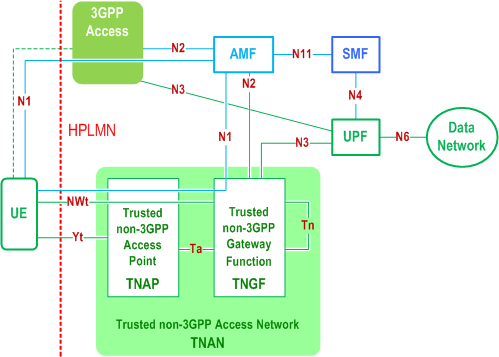
\includegraphics[width=0.5\linewidth]{figs/architecture-for-5g-core-network-with-trusted-non-3gpp-access.png}
    \caption{Architecture for \ac{5GC} with Trusted Non-\acs{3GPP} Access}
    \label{fig:architecture-for-5g-core-network-with-trusted-non-3gpp-access}
\end{figure}

\begin{figure}
    \centering
    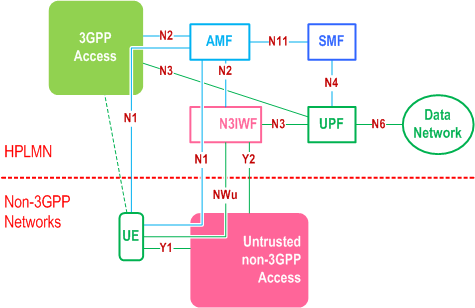
\includegraphics[width=0.5\linewidth]{figs/architecture-for-5g-core-network-with-untrusted-non-3gpp-access.png}
    \caption{Architecture for \ac{5GC} with Untrusted Non-\ac{3GPP} Access}
    \label{fig:architecture-for-5g-core-network-with-untrusted-non-3gpp-access}
\end{figure}

When using non-\ac{3GPP} access, \ac{UE}s establish secure \ac{IPSec} tunnels with the \ac{N3IWF} or \ac{TNGF} to register with the \ac{5GC}. Post-registration, the \ac{NAS} signaling between the \ac{UE} and the core network is protected using the same security mechanisms, N1, as \ac{3GPP} access.

\ac{5G} also enables operators to merge fixed and mobile networks through functional convergence, offering a unified control plane for both wireline and wireless sessions. This approach enhances seamless access-independent services, supports multi-access connectivity, simplifies network operations, unifies technology and training, centralizes subscriber management, extends \ac{5G} core coverage, and broadens fixed access service offerings~\cite{bbf-tr-470-p8}.

\begin{figure}
    \centering
    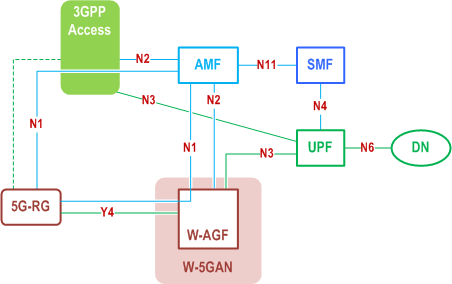
\includegraphics[width=0.5\linewidth]{figs/Architecture for 5G Core Network for 5G-RG with Wireline 5G Access network and NG RAN.png}
    \caption{Architecture for \ac{5GC} for \acs{5G-RG} with \ac{W-5GAN} and \ac{NG-RAN}}
    \label{fig:Architecture for 5G Core Network for 5G-RG with Wireline 5G Access network and NG RAN}
\end{figure}

\ac{W-5GAN}, such as broadband fiber-optic networks, connects to the \ac{5GC} via the \ac{W-AGF} (see Figure \ref{fig:Architecture for 5G Core Network for 5G-RG with Wireline 5G Access network and NG RAN}), using N2 and N3 interfaces for control and user plane functions, respectively. When a \acf{5G-RG}, such as a home router with \ac{5G} capabilities, connects through both \ac{NG-RAN} , like a \ac{5G} cellular tower (e.g. a \ac{FWA} context), and \ac{W-5GAN}, it maintains separate N1 signaling instances for each access. However, a single \ac{AMF} in the same \ac{5GC} serves the \ac{5G-RG}. \ac{NAS} signaling over \ac{W-5GAN} persists even after \acf{PDU} sessions are released ~\cite{23.501-p66}.

\subsection{Device Diversity and Access Options}

As the \ac{5G} network evolves, it's important to recognize that not all devices connected to the network are \ac{5G} capable. While we typically envision \ac{UE} as being \ac{5G}-enabled, \ac{3GPP} has also accounted for a wide range of devices, from legacy systems to non-\ac{5G} capable ones, ensuring that connectivity remains seamless and secure across diverse access points.

\begin{figure}
    \centering
    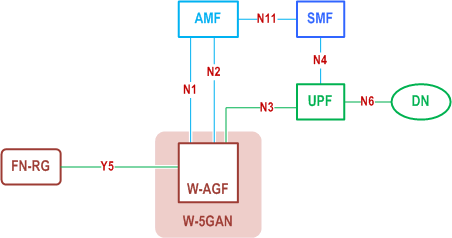
\includegraphics[width=0.5\linewidth]{figs/Architecture for 5G Core Network for FN-RG with Wireline 5G Access network and NG RAN.png}
    \caption{Architecture for \acl{5GC} for \acs{FN-RG} with \ac{W-5GAN} and \ac{NG-RAN}}
    \label{fig:Architecture for 5G Core Network for FN-RG with Wireline 5G Access network and NG RAN}
\end{figure}

For \acp{FN-RG}, such as legacy home routers, connected via \ac{W-5GAN} (see Figure \ref{fig:Architecture for 5G Core Network for FN-RG with Wireline 5G Access network and NG RAN}), the \ac{W-AGF} handles N1 signaling on behalf of the \ac{FN-RG}. \acp{UE}, like smartphones or \ac{IoT} devices, connecting through these gateways can access the \ac{5GC} via either \ac{N3IWF} (untrusted access using Wi-Fi) or \ac{TNGF} (trusted access) depending on the network configuration.

\begin{figure}
    \centering
    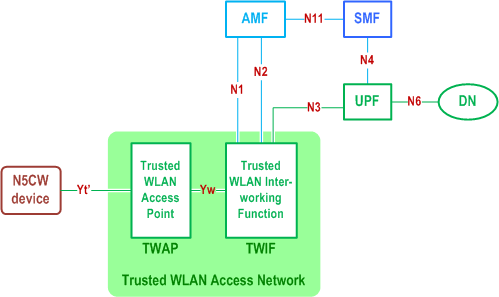
\includegraphics[width=0.5\linewidth]{figs/Architecture for supporting 5GC access from N5CW devices.png}
    \caption{Architecture for supporting \ac{5GC} access from \ac{N5CW} devices}
    \label{fig:Architecture for supporting 5GC access from N5CW devices}
\end{figure}

There are also devices that are not \ac{5G}-capable over \ac{WLAN} access~\cite{23.501-p67}, referred to as \ac{N5CW} devices, cannot support \ac{5GC} \ac{NAS} signaling over \ac{WLAN} but may still operate as \ac{5G} \acp{UE} over \ac{NG-RAN}. \ac{3GPP} provides enhancements for N5CW devices to access \ac{5GC} via trusted \ac{WLAN} access networks (see Figure \ref{fig:Architecture for supporting 5GC access from N5CW devices}), which are a type of \ac{TNAN}, typically using IEEE 802.11 technology. These networks must support specific functions, such as the \ac{TWIF}, which enables \ac{N5CW} devices to register with the \ac{5GC}. When a \ac{N5CW} device performs a \ac{EAP}-based access authentication procedure to connect to a trusted \ac{WLAN} access network, it may simultaneously be registered to an \ac{5GC} of a \ac{PLMN} or \ac{SNPN}. The \ac{TWIF} handles authentication, \ac{AMF} selection, \ac{NAS} protocol communication, and relays user data between the \ac{WLAN} access network and the \ac{5GC}. In this specification, trusted \ac{WLAN} access for \ac{N5CW} devices only supports IP \ac{PDU} sessions.

\subsection{Authentication Flow Across Trusted and Untrusted Networks}
Examining the authentication flows for devices connecting to the \ac{5GC} via non-\ac{3GPP} access networks reveals differences in the mechanisms used for trusted and untrusted accesses.

For untrusted non-\ac{3GPP} access, security is established using \ac{IKEv2} to set up \ac{IPSec} security associations between the \ac{UE} (acting as the \ac{IKE} initiator) and the \ac{N3IWF} (acting as the \ac{IKE} responder). The \ac{UE} and \ac{N3IWF} use a derived key from the \ac{AMF} to complete the authentication process.

In non-roaming scenarios, the home operator (or \ac{HPLMN}) decides whether a non-\ac{3GPP} access network is trusted or untrusted based on its security features, while in roaming scenarios, the decision is made by the \ac{UDM} in the \ac{HPLMN}. This decision applies consistently across all \acp{DN} the \ac{UE} connects to via the same non-\ac{3GPP} access network.

The \ac{UE} stores trusted non-\ac{3GPP} access network information in the \ac{USIM}, which takes priority over the \ac{ME}, the device itself.

For authentication over untrusted non-\ac{3GPP} networks (see Figure \ref{fig:Authentication for untrusted non-3GPP access}), the \ac{UE} uses a vendor-specific \ac{EAP} method called "EAP-5G", which employs the "Expanded" \ac{EAP} type and the \ac{3GPP} Vendor-Id. The \ac{EAP-5G} method is used between the \ac{UE} and \ac{N3IWF} to encapsulate \ac{NAS} messages. If the \ac{UE} requires authentication by the \ac{3GPP} home network, standard authentication methods are applied between the \ac{UE} and the \ac{AUSF}. Whenever possible, the \ac{UE} will reuse the existing \ac{NAS} security context from the \ac{AMF} for authentication~\cite{33.501-p128}.

\begin{figure}
    \centering
    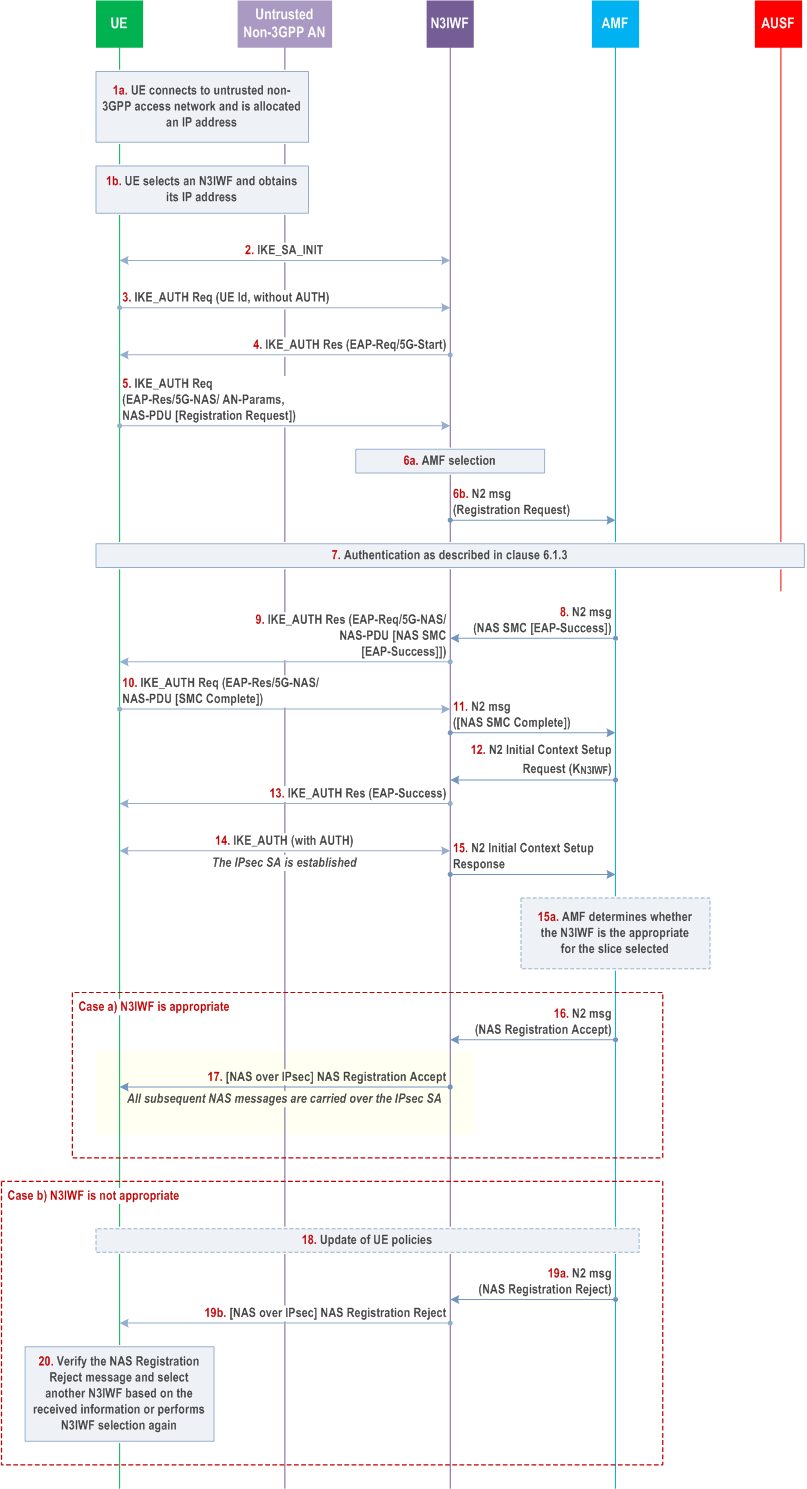
\includegraphics[width=0.75\linewidth]{figs/Authentication for untrusted non-3GPP access.png}
    \caption{Authentication for untrusted non-\ac{3GPP} access}
    \label{fig:Authentication for untrusted non-3GPP access}
\end{figure}

Security for trusted non-\ac{3GPP} access to the \ac{5GC} involves the \ac{UE} registering to the \ac{5GC} via a \ac{TNAN} using the \ac{EAP-5G} procedure, similar to that used for untrusted access (see Figure \ref{fig:Authentication and PDU Session establishment for trusted non-3GPP access_1}, \ref{fig:Authentication and PDU Session establishment for trusted non-3GPP access_2} and \ref{fig:Authentication and PDU Session establishment for trusted non-3GPP access_3} ). The link between the \ac{UE} and the \ac{TNAN} relies on Layer-2 security, making \ac{IPSec} encryption unnecessary between the \ac{UE} and the \ac{TNGF}, though integrity protection is ensured~\cite{33.501-p132}.

During registration, the \ac{TNGF} terminates \ac{EAP-5G} signaling and forwards \ac{NAS} messages to the \ac{5GC}. At the registration's conclusion, an \ac{IPSec SA (NWt)} (an \acl{IPSec SA} managing secure communication parameters at a Network Termination point) is established between the \ac{UE} and \ac{TNGF} to protect \ac{NAS} messages. Additional \acp{IPSec SA} are created during \ac{PDU} session establishment for user plane transport. Security policies, determined by the home operator, define whether non-\ac{3GPP} access is trusted based on security domains or other considerations.

For trusted non-\ac{3GPP} access authentication, key differences from untrusted access include avoiding \ac{IKEv2} encapsulation for \ac{EAP-5G} packets, utilizing \ac{5G-GUTI} or \ac{SUCI} for \ac{UE} identity, and deriving keys like $K_TNGF$ and $K_TNAP$ for secure communication. These keys are shared between the \ac{AMF}, \ac{TNGF}, and \ac{TNAP} to establish secure communication flows.

\begin{figure}
    \centering
    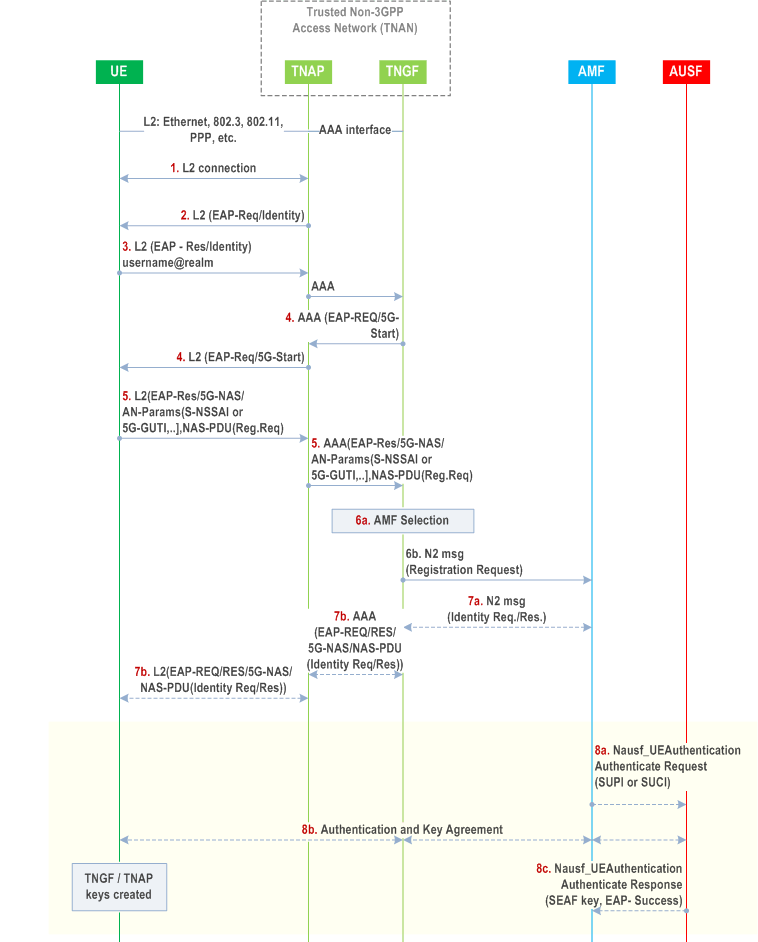
\includegraphics[width=0.75\linewidth]{figs/Authentication and PDU Session establishment for trusted non-3GPP access_1.png}
    \caption{Authentication and \ac{PDU} Session establishment for trusted non-\ac{3GPP} access}
    \label{fig:Authentication and PDU Session establishment for trusted non-3GPP access_1}
\end{figure}

\begin{figure}
    \centering
    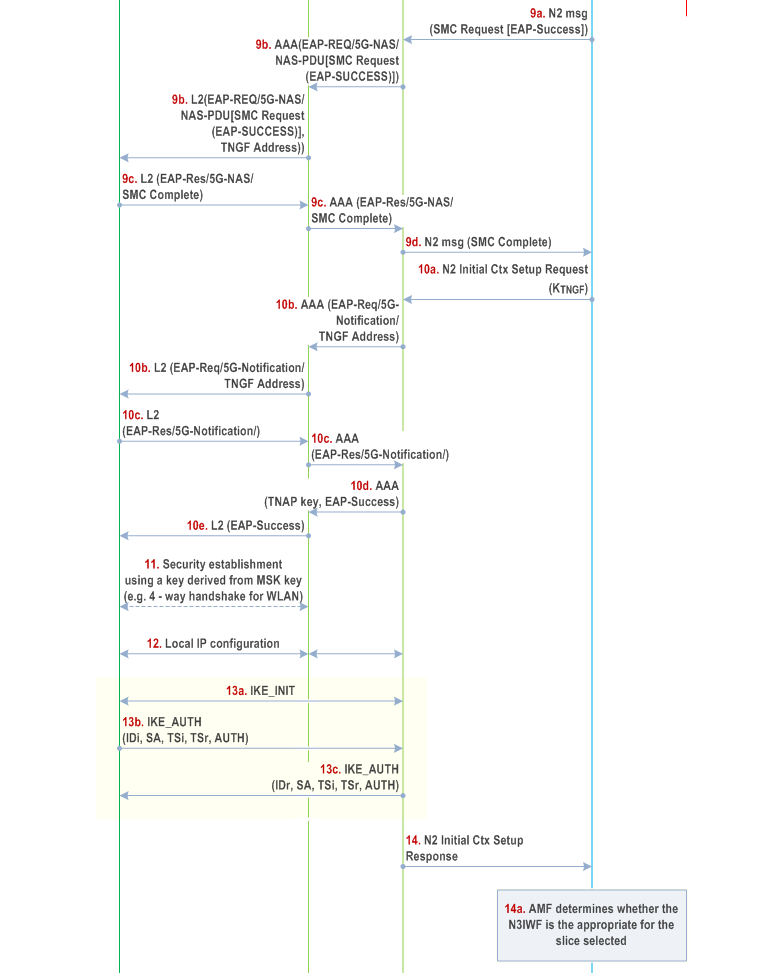
\includegraphics[width=0.75\linewidth]{figs/Authentication and PDU Session establishment for trusted non-3GPP access_2.png}
    \caption{Authentication and \ac{PDU} Session establishment for trusted non-\ac{3GPP} access (continuation)}
    \label{fig:Authentication and PDU Session establishment for trusted non-3GPP access_2}
\end{figure}

\begin{figure}
    \centering
    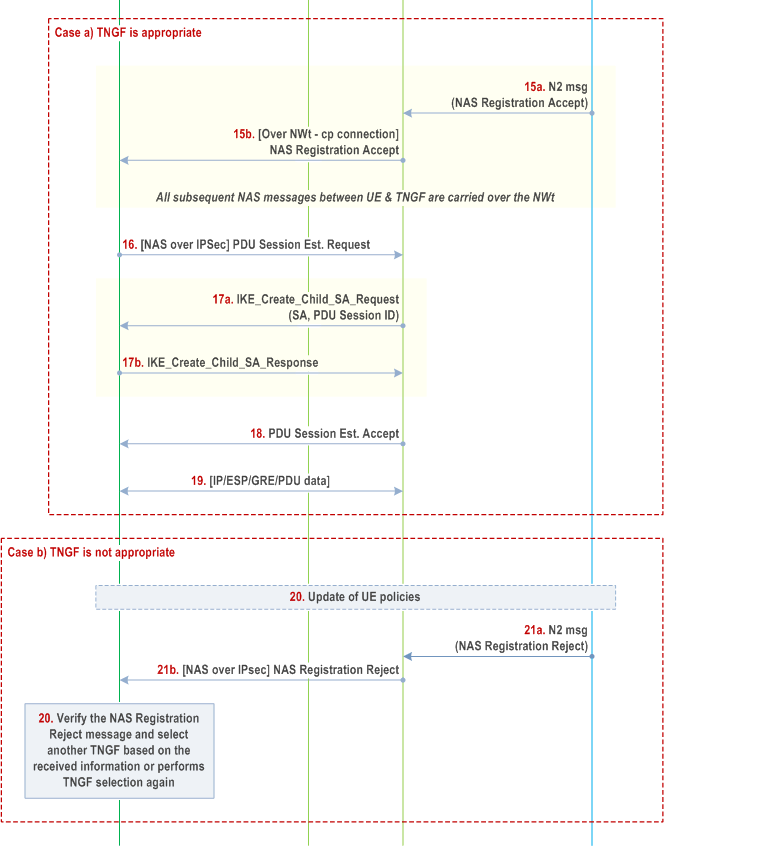
\includegraphics[width=0.75\linewidth]{figs/Authentication and PDU Session establishment for trusted non-3GPP access_3.png}
    \caption{Authentication and \ac{PDU} Session establishment for trusted non-\ac{3GPP} access (continuation)}
    \label{fig:Authentication and PDU Session establishment for trusted non-3GPP access_3}
\end{figure}

\section{Device Support Behind Wireline}

As we shift focus from non-\ac{3GPP} access networks, it’s important to examine wireline access, which is crucial for connecting home devices like laptops, smart TVs, and \ac{IoT} devices to the \ac{5GC}. Many of these devices rely on wireline connections, often through home routers like \ac{5G-RG} and \ac{FN-RG}~\cite{33.501-p139}, to access the \ac{5G} network. Understanding how wireline access works is vital, as it bridges the gap for devices without full \ac{5G} capabilities, ensuring seamless integration across both fixed and wireless environments.

For instance, in a smart home, a \ac{5G-RG} might connect to the \ac{5GC} using fiber or \ac{FWA}, while an enterprise could use an \ac{FN-RG} for secure, high-speed access via wireline networks. The connection between the \ac{RG} and \ac{W-5GAN} leverages \ac{5G} security frameworks, similar to wireless setups. However, roaming is not supported for these entities or the devices they serve. In specific configurations, additional \ac{EAP} methods can be used to ensure secure authentication, enabling devices like remote workstations to securely access the \ac{5GC}. This enables seamless and secure integration of \ac{5G} across fixed and wireless environments.

The \ac{5G-RG} supports \ac{5GC} connections via \ac{NG-RAN}, \ac{W-5GAN}, or both, with registration processes varying by access type~\cite{23.316-p29}~\cite{23.316-p37}. As the \ac{5G-RG} is treated as a \ac{UE} by the \ac{5GC}, it uses the standard authentication framework, including \ac{5G-AKA} and \ac{EAP-AKA'}. For \ac{W-5GAN} connections, \ac{W-CP} protocol stack messages encapsulate \ac{NAS} signaling. In contrast, the \ac{FN-RG} connects exclusively via \ac{W-5GAN} and relies on the \ac{W-AGF} to handle N1 signaling on its behalf. The \ac{W-AGF} provides connectivity to the \ac{5GC} via N2 and N3 interfaces and can authenticate the \ac{FN-RG} based on local policies. Secure protocols like \ac{NDS/IP} or \ac{DTLS} establish mutual trust between the wireline operator managing the \ac{W-5GAN} and the \ac{PLMN} operator managing the \ac{5GC}~\cite{23.316-p41}.

Devices such as \ac{N5CW} occupy a middle ground. While they lack full \ac{5G} functionality over \ac{WLAN}, they can still register with the \ac{5GC}, establish \ac{PDU} sessions, and authenticate using \ac{3GPP} credentials (\ac{USIM}). These devices may function as regular \acp{UE} when connected via cellular networks, unlike \ac{N5GC} devices, which lack \ac{5G}-specific capabilities~\cite{33.501-p279}.

In wireline access, gateways like the \ac{5G-RG} and \ac{FN-RG} enable connectivity for devices that cannot independently handle \ac{NAS} signaling or derive \ac{5G} keys. For example, the \ac{W-AGF} manages registration on behalf of \ac{FN-RG} devices and ensures secure communication with the \ac{5GC}. For \ac{N5GC} devices connecting via \ac{CRG}, the \ac{SUPI} includes a network-specific identifier (\ac{NAI}), and the \ac{W-AGF} derives the \ac{SUCI} from the \ac{EAP}-Identity message, passing it to the \ac{AMF} for secure identification~\cite{23.316-p23}.

This architecture enables a diverse range of devices, from \ac{IoT} sensors to legacy systems, to benefit from \ac{5G} connectivity without requiring full \ac{5G} capabilities. It highlights the critical role of wireline access in achieving seamless convergence across fixed and wireless network environments while maintaining robust security.

\subsection{\acs{5GC} Registration Process for \acs{N5GC} Devices}

In isolated \ac{5G} networks with wireline access, \ac{N5GC} devices can access the \ac{5GC} through a structured process involving \ac{EAP}-based authentication. Each \ac{N5GC} device is treated as an individual entity with its own subscription record in the \ac{UDM}/\ac{UDR}, distinct from the subscription record of the \ac{CRG}. The \ac{CRG} operates in L2 bridge mode, forwarding traffic from connected \ac{N5GC} devices to the \ac{W-AGF} for further processing and registration.

\begin{figure}
    \centering
    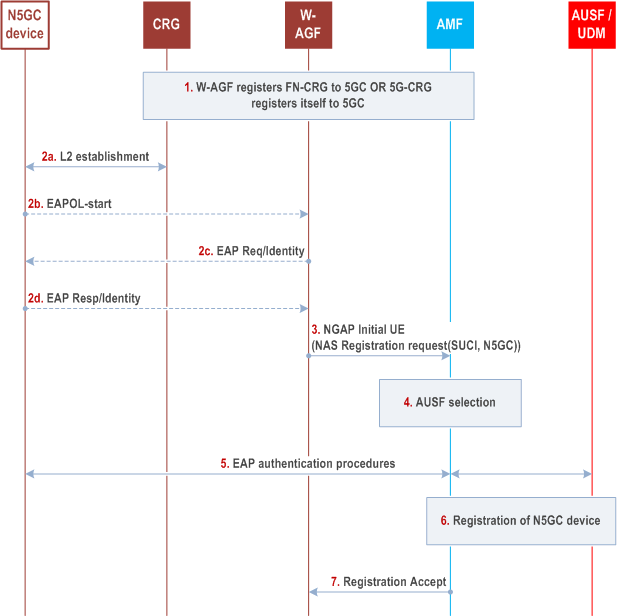
\includegraphics[width=0.75\linewidth]{figs/5GC registration of Non-5GC device.png}
    \caption{\ac{5GC} registration of \ac{N5GC} device}
    \label{fig:5GC registration of Non-5GC device}
\end{figure}

The process begins with the registration of the \ac{CRG} to the \ac{5GC} (the flow is shown in Figure \ref{fig:5GC registration of Non-5GC device}). This enables the \ac{CRG} to act as a bridge, facilitating communication between \ac{N5GC} devices and the \ac{W-AGF}. Once this setup is in place, authentication is triggered when the \ac{CRG} forwards traffic from an \ac{N5GC} device. This occurs either through the reception of an \textit{\ac{EAPOL}-Start} frame sent by the \ac{N5GC} device or when the \ac{W-AGF} detects traffic from an unknown \ac{MAC} address. The \ac{N5GC} device responds by sending an \textit{\ac{EAP}-Response/Identity} message containing its \ac{NAI}, formatted as \texttt{username@realm}.

The \ac{W-AGF} then acts on behalf of the \ac{N5GC} device to initiate its registration with the \ac{5GC}. It constructs and sends a \textit{\ac{NAS} Registration Request} to the \ac{AMF}, including a \ac{SUCI} derived from the \ac{NAI}. This registration explicitly indicates that the device lacks native \ac{5G} capabilities. The \ac{W-AGF} establishes separate \ac{NGAP} connections for each \ac{N5GC} device over the N2 interface, enabling distinct communication channels for every device.

Authentication of the \ac{N5GC} device is carried out by the \ac{AUSF} using \ac{EAP}-based methods. Once the device successfully authenticates, the \ac{AUSF} provides the relevant security information to the \ac{AMF}, including the \ac{SUPI} derived from the \ac{NAI}. This \ac{SUPI} uniquely identifies the \ac{N5GC} device within the \ac{5GC} ecosystem, ensuring individual accountability and secure operation.

Following successful authentication, the \ac{AMF} completes additional registration procedures. If a \ac{PEI} is required, the \ac{W-AGF} uses the \ac{MAC} address of the \ac{N5GC} device, with an option to encode it in IEEE \ac{EUI-64} format depending on operator policy. Once registration is finalized, the \ac{W-AGF} communicates the \textit{Registration Accept} message to the \ac{N5GC} device, marking the completion of the process.

After registration, the \AC{W-AGF} establishes a single \ac{PDU} session for each \ac{N5GC} device, ensuring each device is assigned its own unique data session within the \ac{5GC} while accounting for the device's limitations. This ensures secure and individualized connectivity. Additionally, the \ac{W-AGF} manages \ac{NGAP} connections, ensuring that if the \ac{NGAP} connection for a \ac{CRG} is released, all associated \ac{N5GC} device connections are also terminated. The \ac{CRG} continues to operate as an \ac{FN-CRG}, supporting seamless communication for connected devices~\cite{23.316-p25}.

\begin{figure}
    \centering
    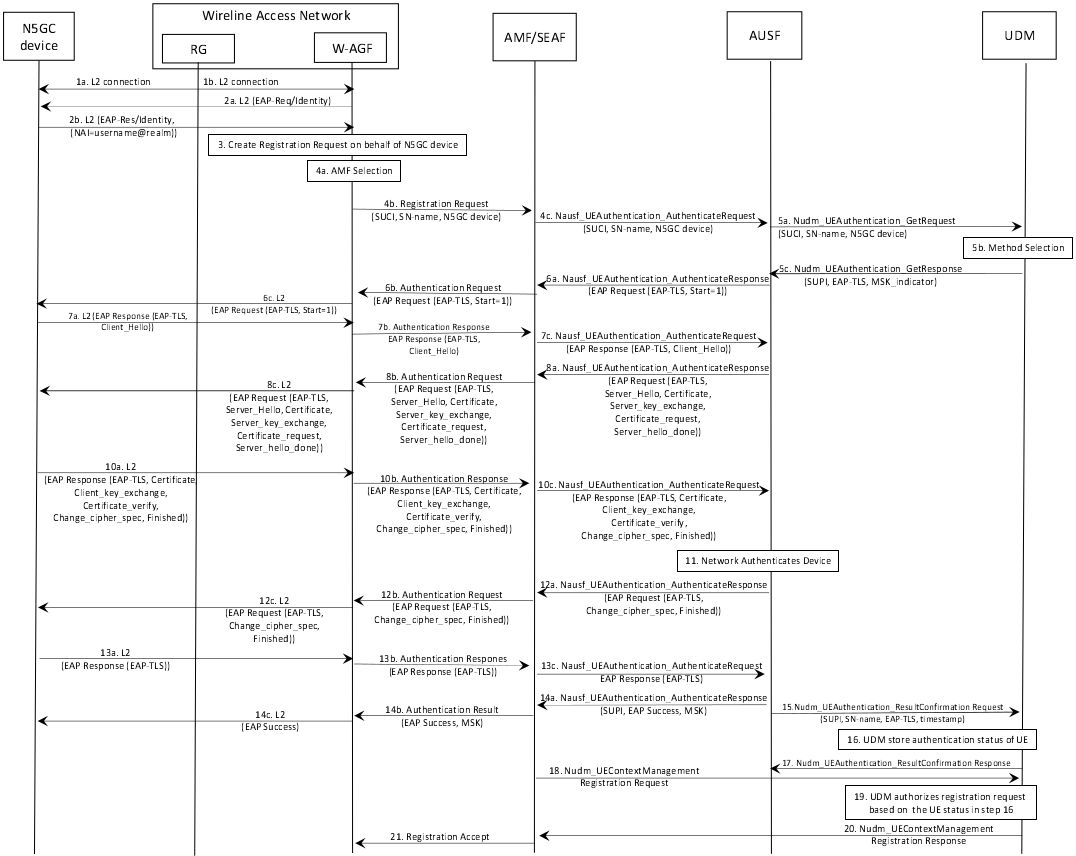
\includegraphics[width=0.75\linewidth]{figs/Detailed registration and authentication flow of a non-5G capable device to the 5GC.png}
    \caption{Detailed registration and authentication flow of a \ac{N5GC} device to the \ac{5GC}}
    \label{fig:Detailed registration and authentication flow of a non-5G capable device to the 5GC}
\end{figure}

In Annex 0 of TS 33.501, we can get more detail regarding this registration and authentication process (see Firgure \ref{fig:Detailed registration and authentication flow of a non-5G capable device to the 5GC})~\cite{33.501-p279}.

\subsection{\ac{N5GC} and \acs{NAUN3} devices}

A \acf{NAUN3} device does not support \ac{NAS} signalling, is connected to \ac{5GC} via a \ac{RG} and does not support authentication with the \ac{5GC}~\cite{23.316-p10}.

\ac{NAUN3} devices, which cannot be authenticated by the \ac{5GC}, may be locally authenticated by the \ac{5G-RG} using methods like pre-shared secrets. Examples of pre-shared secrets include Wi-Fi passphrases for \acp{SSID}, \ac{PIN} codes, or static security keys configured during device setup. Differentiated services, including \ac{QoS} and network slicing, can be applied to these devices through \acp{CGID} (see Figure \ref{fig:NAUN3 devices behind 5G-RG based on connectivity groups}).

\begin{figure}
    \centering
    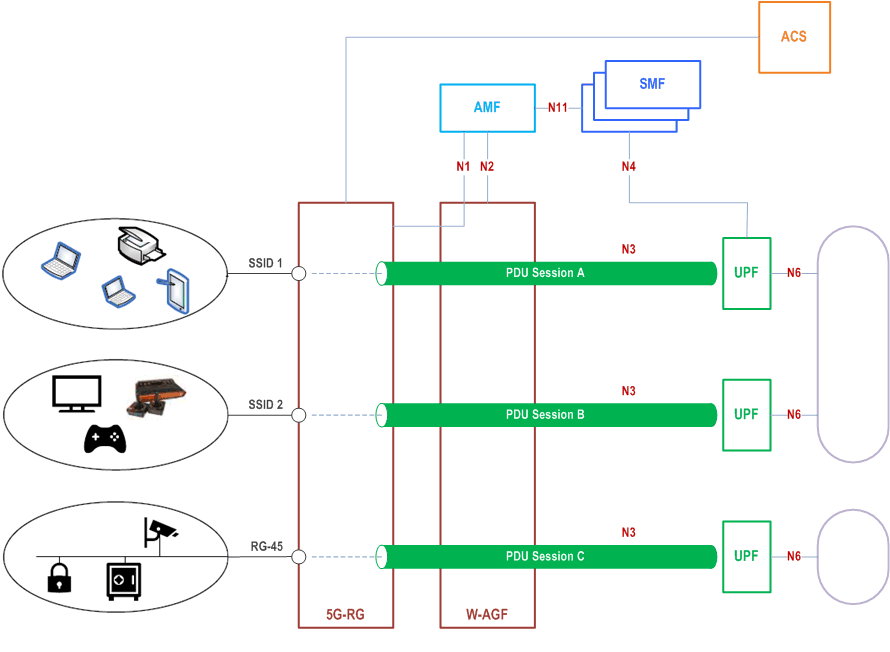
\includegraphics[width=0.75\linewidth]{figs/NAUN3 devices behind 5G-RG based on connectivity groups.png}
    \caption{NAUN3 devices behind \ac{5G-RG} based on connectivity groups}
    \label{fig:NAUN3 devices behind 5G-RG based on connectivity groups}
\end{figure}

Each \ac{CGID} corresponds to a specific physical or virtual port on the \ac{5G-RG}, such as Ethernet ports, \ac{WLAN} \acp{SSID}, or \acp{VLAN}. Devices connected to the same logical port are considered part of the same \ac{CGID}, and each \ac{CGID} maps to a separate \ac{PDU} Session established by the \ac{5G-RG} to manage their traffic.

The \ac{5G-RG} is configured with port information, such as \acp{VLAN} and \ac{SSID}, via standardized protocols like TR-69, TR-360, and TR-181. \ac{URSP} rules are provided to the \ac{5G-RG} to define how \acp{CGID} are mapped to \ac{PDU} Session parameters, such as the \ac{DNN} and \ac{S-NSSAI}. These mappings determine how traffic is routed and which network slice the devices use. For instance, a home office \ac{CGID} might map to a \ac{DNN} providing enterprise services and an \ac{S-NSSAI} prioritizing low latency for work-related tasks.

Charging and \ac{QoS} differentiation for \ac{NAUN3} devices can be implemented through \ac{PCC} rules. These rules define service flows tied to specific \ac{PDU} Sessions, enabling detailed traffic management and billing policies. Additionally, isolation of devices using a specific \ac{CGID} into a separate network slice (associated with an \ac{S-NSSAI}) can provide enhanced security and service customization. For example, devices in a child’s \ac{CGID} could be isolated into a network slice with strict content filtering and bandwidth limitations~\cite{23.316-p27}.

The main difference between \ac{NAUN3} and \ac{N5GC} devices lies in their capabilities and how they interact with the \ac{5GC}, here is a summary of what we've seen soo far (also represented in Table \ref{tab:Key Differences between NAUN3 and N5GC devices}):

\begin{itemize}
    \item {
        \textbf{\ac{NAUN3} Devices}
        \begin{itemize}
            \item {
                \textbf{Authentication}: They cannot be authenticated by the \ac{5GC}. Instead, they rely on local authentication mechanisms provided by the \ac{5G-RG} (e.g., Wi-Fi passphrases, \acp{PIN}, or pre-shared keys).
            }
            \item {
                \textbf{Connection}: \ac{NAUN3} devices connect through the \ac{5G-RG}, which maps their traffic to \ac{PDU} Sessions and handles aspects like \ac{QoS} and network slicing (e.g., via \ac{S-NSSAI}).
            }
            \item {
                \textbf{Subscription Records}: \ac{NAUN3} devices do not have subscription records in the \ac{5GC} and operate entirely under the configuration and policies of the \ac{5G-RG}.
            }
            \item {
                \textbf{Purpose}: They are typically legacy or \ac{IoT} devices that do not need direct \ac{5GC} access but require differentiated services provided via local configuration and mapping, and need to be connected via Layer 2 to \ac{5G} devices via extended slices.
            }
            \item {
                \textbf{Example}: A smart home appliance connected to the \ac{5G-RG} via Wi-Fi using a pre-shared key, with its traffic routed through a dedicated network slice.
            }
        \end{itemize}    
    }
    \item {
        \textbf{\ac{N5GC} Devices}
        \begin{itemize}
            \item {
                \textbf{Authentication}: They can be authenticated by the \ac{5GC} using \ac{EAP}-based authentication with the help of the \ac{W-AGF}, which acts as an intermediary.
            }
            \item {
                \textbf{Connection}: \ac{N5GC} devices connect to the \ac{5GC} through wireline access (e.g., fiber or \ac{DSL}) and use the \ac{W-AGF} to handle their registration, authentication, and session management.
            }
            \item {
                \textbf{Subscription Records}: Each \ac{N5GC} device has its own unique subscription record in the \ac{UDM}/\ac{UDR}, separate from the subscription record of the \ac{CRG}.
            }
            \item {
                \textbf{\ac{NGAP} Connections}: The \ac{W-AGF} establishes separate \ac{NGAP} connections for each \ac{N5GC} device over the N2 interface to the \ac{AMF}. This enables individual session and mobility management for each device.
            }
            \item {
                \textbf{Purpose}: \ac{N5GC} devices extend \ac{5GC} services to fixed network devices that do not possess \ac{5G} capabilities.
            }
            \item {
                \textbf{Example}: A desktop computer connected to the \ac{5GC} via fiber access and authenticated using \ac{EAP} over the \ac{W-AGF}.
            }
        \end{itemize}    
    }
\end{itemize}

In summary, \ac{NAUN3} devices operate entirely locally, with no interaction with the \ac{5GC}, while \ac{N5GC} devices leverage intermediaries like the \ac{W-AGF} to authenticate and establish \ac{PDU} Sessions with the \ac{5GC}, maintaining unique subscription records and dedicated \ac{NGAP} connections.